\subsection{Semantic agreement and the cost of maintaining justifications}\label{sec:res-systems}
\begin{sidewaystable}\centering\small
\caption{Incremental justification maintenance vs symbolic replay of the same semantics on the same streams and queries (no LLM). CPU seconds per stream (process time), query latency mean / p95 / max in ms, peak traced memory in MB; $r$ = queries per observation. Answers agree on every query (last column: disagreements / answers). Scale rows: generated streams with $m$ reports per key and horizon $T$ days, $r=1$.}\label{tab:sys}
\begin{tabular}{llrrrrrrrr}
\toprule
Workload & System & CPU total & CPU write & lat.\ mean & p95 & max & mem & recomputes & disagree \\
\midrule
Setting 1, r=0.1 & incremental & 0.33 & 0.32 & 0.4 & 1.0 & 12 & 1.0 & 136 & 0/799 \\
 & replay cold & 0.03 & 0.00 & 2.6 & 6.7 & 61 & 0.1 & 17 &  \\
 & replay lazy & 0.04 & 0.00 & 2.6 & 6.8 & 98 & 0.2 & 17 &  \\
\addlinespace[2pt]
Setting 1, r=0.33 & incremental & 0.32 & 0.31 & 0.4 & 1.2 & 10 & 0.9 & 136 & 0/2637 \\
 & replay cold & 0.11 & 0.00 & 2.6 & 9.2 & 69 & 0.3 & 57 &  \\
 & replay lazy & 0.11 & 0.00 & 2.5 & 9.4 & 73 & 0.5 & 56 &  \\
\addlinespace[2pt]
Setting 1, r=1.0 & incremental & 0.36 & 0.32 & 0.4 & 1.5 & 57 & 1.0 & 136 & 0/7974 \\
 & replay cold & 0.32 & 0.00 & 2.4 & 11.0 & 79 & 0.5 & 173 &  \\
 & replay lazy & 0.32 & 0.00 & 2.4 & 11.1 & 117 & 1.3 & 165 &  \\
\addlinespace[2pt]
Setting 1, r=3.0 & incremental & 0.46 & 0.32 & 0.3 & 1.6 & 40 & 1.2 & 136 & 0/23922 \\
 & replay cold & 0.93 & 0.00 & 2.3 & 11.7 & 85 & 0.7 & 520 &  \\
 & replay lazy & 0.87 & 0.00 & 2.2 & 11.1 & 81 & 3.2 & 449 &  \\
\addlinespace[2pt]
scale $m$=10, $T$=120, $r$=1.0 & incremental & 2.15 & 1.89 & 1.3 & 7.0 & 56 & 8.5 & 206 & 0/992 \\
 & replay cold & 3.16 & 0.00 & 15.7 & 91.2 & 487 & 1.8 & 248 &  \\
 & replay lazy & 3.09 & 0.00 & 15.4 & 82.5 & 481 & 11.0 & 240 &  \\
\addlinespace[2pt]
scale $m$=10, $T$=60, $r$=1.0 & incremental & 0.97 & 0.86 & 0.8 & 1.9 & 57 & 4.1 & 134 & 0/668 \\
 & replay cold & 1.10 & 0.00 & 8.3 & 31.5 & 597 & 1.5 & 176 &  \\
 & replay lazy & 1.01 & 0.00 & 7.7 & 29.7 & 597 & 3.9 & 167 &  \\
\addlinespace[2pt]
scale $m$=13, $T$=60, $r$=1.0 & incremental & 3.72 & 3.61 & 0.9 & 1.8 & 215 & 22.4 & 138 & 0/686 \\
 & replay cold & 1.66 & 0.00 & 12.5 & 34.3 & 2553 & 4.2 & 183 &  \\
 & replay lazy & 1.62 & 0.00 & 12.2 & 32.2 & 2475 & 7.2 & 174 &  \\
\addlinespace[2pt]
scale $m$=7, $T$=120, $r$=1.0 & incremental & 0.57 & 0.48 & 0.6 & 2.7 & 11 & 1.9 & 166 & 0/800 \\
 & replay cold & 0.66 & 0.00 & 4.2 & 19.6 & 73 & 0.7 & 227 &  \\
 & replay lazy & 0.68 & 0.00 & 4.4 & 18.0 & 104 & 2.7 & 218 &  \\
\addlinespace[2pt]
scale $m$=7, $T$=240, $r$=1.0 & incremental & 0.79 & 0.61 & 0.9 & 4.1 & 16 & 2.9 & 187 & 0/934 \\
 & replay cold & 1.38 & 0.00 & 7.4 & 31.7 & 108 & 1.1 & 259 &  \\
 & replay lazy & 1.42 & 0.00 & 7.6 & 31.3 & 177 & 5.3 & 254 &  \\
\addlinespace[2pt]
scale $m$=7, $T$=60, $r$=1.0 & incremental & 0.34 & 0.30 & 0.3 & 1.4 & 11 & 1.1 & 129 & 0/618 \\
 & replay cold & 0.24 & 0.00 & 2.0 & 8.2 & 45 & 0.4 & 161 &  \\
 & replay lazy & 0.24 & 0.00 & 2.0 & 8.3 & 49 & 1.0 & 153 &  \\
\addlinespace[2pt]
\bottomrule
\end{tabular}
\end{sidewaystable}
\begin{figure}[t]\centering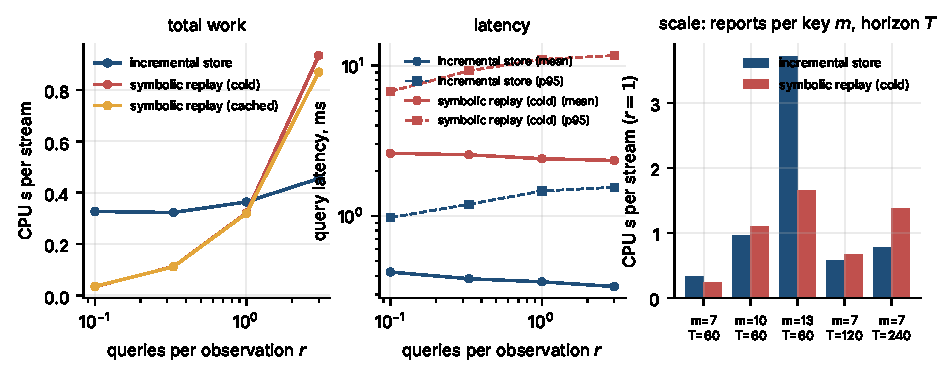
\includegraphics[width=\textwidth]{figures/systems.pdf}
\caption{Incremental maintenance vs symbolic replay on the same streams and queries (no LLM). Left: CPU per stream against the query/observation ratio; replay is cheaper below $r\approx1$, maintenance above. Centre: query latency (mean and p95). Right: total CPU at $r=1$ as reports per key $m$ and horizon $T$ grow; the store's per-write enumeration dominates at $m=13$.}\label{fig:systems}
\end{figure}
The first result is an equivalence, stated by field. \pal{} and symbolic replay execute the same semantics on the same evidence and must return the same status, assertion and alternatives; on every query of every setting they now do: the 30{,}272 queries of Setting 1 (both equal the oracle), the 6{,}737 of Setting 2, the 714 of Setting 3, the 994 of the Sonnet subset, and the \sysAnswers{} queries of the workload study in Table~\ref{tab:sys}, with \sysDisagree{} disagreements on those three fields. The provenance lists differ on 2.3\% of Setting 2 and 5.3\% of Setting 3 queries, the store citing the observations of the pinned key versions and replay the observations on justification paths, which is why their provenance precision differs by about a point; the full contract JSON is therefore not identical, the scored fields are. They did not at first: 18 of 6{,}737 Setting 2 answers differed, all of one kind---an extracted correction whose entity and value the extractor had swapped landed on a different key from its target, replay applied the same-origin withdrawal (A-SELF) globally and the store applied it only on the correction's own key. The fix is recorded as a dated deviation; the structured systems were re-scored from the cached extractions, which moved \pal's Setting 2 warranted downstream accuracy from 0.953 to \sTwoPalWarr, direct accuracy from 0.993 to 0.996, resolvable accuracy from 0.975 to 0.976 and commitment from 0.082 to 0.080, and left the LLM rows untouched. We mention it because the reviewer-visible discrepancy of three tenths of a point was a real bug, and because it shows what the equivalence check is for.

The second result is the cost, which the subtitle of an earlier draft asked about and which Table~\ref{tab:sys} and Figure~\ref{fig:systems} answer. At the generator's default scale (133 observations per stream, at most seven reports per key) replay does \emph{less} total work than maintenance when queries are rarer than observations ($r=0.1$: \sysRpOneRepCpu{} vs \sysRpOneIncCpu{}~s per stream; $r=1$: \sysROneRepCpu{} vs \sysROneIncCpu{}), and more when they are more frequent ($r=3$: \sysRThreeRepCpu{} vs \sysRThreeIncCpu{}); the crossing is workload-dependent: interpolating the two measured points around it at default scale puts it near 1.1 queries per observation, with no repeated runs to attach an uncertainty to. Longer histories move it in maintenance's favour (240-day horizon at $r=1$: \sysTTwoFortyRepCpu{} vs \sysTTwoFortyIncCpu{}), more reports per key move it against: at 13 reports per key the per-write enumeration of interpretations costs \sysMThirteenIncCpu{}~s against \sysMThirteenRepCpu{} for replay and \sysMThirteenIncMem{}~MB of peak memory against \sysMThirteenRepMem{}, because the store re-enumerates a key's $2^n$ labelings on every write while replay enumerates only the keys a query touches. What maintenance buys at every scale is measured latency: \sysROneIncLat{}~ms per query against \sysROneRepLat{} at $r=1$, p95 \sysROneIncPNN{} against \sysROneRepPNN{}, and a worst case of \sysMThirteenIncMax{}~ms against \sysMThirteenRepMax{}~ms at 13 reports per key. The summary is that write-time justification maintenance gives the same answers with lower measured query latency, saves total work only when queries are at least as frequent as observations or histories are long, and has a write cost exponential in reports per key that bounds its use without a smarter per-key representation. None of this involves an LLM; it is the systems question separated from the adjudication question. Method: one process on a 2-vCPU Intel Xeon 2.80\,GHz container (Python 3.13, Linux), CPU time by \texttt{time.process\_time}, each (stream, ratio) cell run once in the order incremental, cold replay, cached replay on a fresh copy of the stream, default garbage collection, memory as \texttt{tracemalloc} peak traced allocation (not resident memory); 60 Setting 1 streams per ratio and 5 generated streams per scale cell; latency distributions are over queries, the maxima are single observations, and no interval is attached to the CPU totals.

\subsection{Setting 1: structured streams, gold dependencies}\label{sec:res-s1}
\begin{sidewaystable}\centering\footnotesize\setlength{\tabcolsep}{3.5pt}
\caption{Setting 1 (structured streams, gold dependencies, no LLM; 500 streams). Stream-level means with 95\% cluster-bootstrap intervals.}\label{tab:s1}
\begin{tabular}{lcccccccc}
\toprule
System & Warr.\ downstream & Warr.\ direct & Resolvable & Unresolved & Commit rate$\downarrow$ & Unsupp.\ prop.$\downarrow$ & Prov.\ P & Prov.\ R \\
\midrule
\textsc{Palimpsest} & 1.000 {\tiny[1.00,1.00]} & 1.000 {\tiny[1.00,1.00]} & 1.000 {\tiny[1.00,1.00]} & 1.000 {\tiny[1.00,1.00]} & 0.000 {\tiny[0.00,0.00]} & 0.000 {\tiny[0.00,0.00]} & 0.990 {\tiny[0.99,0.99]} & 0.993 {\tiny[0.99,0.99]} \\
\quad no propagation & 0.794 {\tiny[0.78,0.81]} & 1.000 {\tiny[1.00,1.00]} & 0.933 {\tiny[0.93,0.94]} & 0.962 {\tiny[0.96,0.97]} & 0.002 {\tiny[0.00,0.00]} & 0.017 {\tiny[0.01,0.02]} & 0.981 {\tiny[0.98,0.98]} & 0.989 {\tiny[0.99,0.99]} \\
\quad forced commit & 1.000 {\tiny[1.00,1.00]} & 1.000 {\tiny[1.00,1.00]} & 1.000 {\tiny[1.00,1.00]} & 0.042 {\tiny[0.04,0.05]} & 0.776 {\tiny[0.76,0.79]} & 0.090 {\tiny[0.08,0.10]} & 0.992 {\tiny[0.99,0.99]} & 0.775 {\tiny[0.77,0.78]} \\
Log + rule adjudicator & 1.000 {\tiny[1.00,1.00]} & 1.000 {\tiny[1.00,1.00]} & 1.000 {\tiny[1.00,1.00]} & 1.000 {\tiny[1.00,1.00]} & 0.000 {\tiny[0.00,0.00]} & 0.000 {\tiny[0.00,0.00]} & 1.000 {\tiny[1.00,1.00]} & 1.000 {\tiny[1.00,1.00]} \\
Temporal DB & 0.807 {\tiny[0.79,0.82]} & 0.909 {\tiny[0.89,0.92]} & 0.907 {\tiny[0.90,0.91]} & 0.000 {\tiny[0.00,0.00]} & 0.848 {\tiny[0.84,0.86]} & 0.105 {\tiny[0.09,0.12]} & 0.950 {\tiny[0.95,0.95]} & 0.341 {\tiny[0.33,0.35]} \\
Always abstain & 0.000 {\tiny[0.00,0.00]} & 0.000 {\tiny[0.00,0.00]} & 0.000 {\tiny[0.00,0.00]} & 0.393 {\tiny[0.38,0.41]} & 0.000 {\tiny[0.00,0.00]} & 0.075 {\tiny[0.06,0.09]} & 0.507 {\tiny[0.50,0.51]} & 0.739 {\tiny[0.73,0.75]} \\
Always commit & 0.438 {\tiny[0.42,0.46]} & 0.970 {\tiny[0.96,0.98]} & 0.770 {\tiny[0.76,0.78]} & 0.000 {\tiny[0.00,0.00]} & 0.793 {\tiny[0.78,0.81]} & 0.157 {\tiny[0.14,0.17]} & 0.939 {\tiny[0.93,0.94]} & 0.284 {\tiny[0.28,0.29]} \\
\bottomrule
\end{tabular}
\end{sidewaystable}
Table~\ref{tab:s1} reports all systems on 500 streams (\sOneAnswers{} scored answers per system; Appendix~\ref{app:tables} gives the per-slot breakdown and the dispute-policy sensitivity). \pal{} and replay reproduce the oracle on every query. Removing retraction propagation costs $\sOnePropEffect$ points $[\sOnePropLo, \sOnePropHi]$ on warranted downstream queries (paired over \sOnePropN{} streams) and nothing on direct ones: ordinary belief updating handles the retracted key, only propagation handles its consequences. The forced-commit variant keeps perfect resolvable accuracy while committing on \sOneCommitRate\% of unresolved slots and changing downstream answers after non-warranted events $\sOneCommitUnsup$ points $[\sOneCommitUnsupLo, \sOneCommitUnsupHi]$ more often. The references split as required (always-abstain: \sOneAbstainRes{} resolvable / \sOneAbstainUnres{} unresolved; always-commit: \sOneCommitRes{} / \sOneCommitUnres{}); always-commit scores below one on unresolved slots because yes/no \emph{erroneous} questions and \texttt{reported} slots are answered by rule, not by recency. The temporal DB loses \sOneTdbWarr{} points on warranted downstream queries and commits on \sOneTdbCommit\% of unresolved slots. These are validation results on a benchmark whose generator and system share an author: they establish that the instruments discriminate, not that any hypothesis holds.

\subsection{When is recency right?}\label{sec:res-regime}
\begin{sidewaystable}\centering\small
\caption{When is recency right? Value queries on single-valued keys of 200 fresh generated streams (seeds 20000--20199), classified from the hidden generator labels by what the latest report on the key is; the same queries are scored under P0c and under the self-update variant P0cSU (paired). Accuracy against the hidden world value; LWW = last-write-wins by report time; valid = by valid-time anchor (temporal DB); abst.\ = abstention rate; wrong commit = committed to a value other than the world's (not a transition); argmax = support-ranked commitment on unresolved slots (P0c). $^\dagger$Poisoning row from 60 attack streams (rate 0.2, low channel), P0c only; its last column is the share of queries committed to the injected value (LWW: 1.00). Setting 1 (500 streams) gives the same picture (Appendix~\ref{app:tables}).}\label{tab:regime}
\begin{tabular}{lrcccccccccc}
\toprule
Regime (latest report) & $n$ & LWW & valid & P0c world & P0c abst. & P0c wrong commit & P0cSU world & P0cSU abst. & P0cSU wrong commit & argmax & injected \\
\midrule
self-update (same origin, latest true) & 53 & 0.96 & 0.96 & 0.68 & 0.32 & 0.00 & 0.96 & 0.00 & 0.04 & 0.94 & -- \\
multi-source update (latest true) & 854 & 0.92 & 0.92 & 0.71 & 0.24 & 0.04 & 0.73 & 0.23 & 0.05 & 0.85 & -- \\
earlier report erroneous, latest true & 1427 & 0.92 & 0.90 & 0.56 & 0.41 & 0.04 & 0.57 & 0.39 & 0.04 & 0.84 & -- \\
delayed report (latest true but older) & 75 & 0.12 & 0.32 & 0.11 & 0.63 & 0.27 & 0.13 & 0.59 & 0.28 & 0.35 & -- \\
latest erroneous, low-trust source & 192 & 0.03 & 0.09 & 0.01 & 0.95 & 0.04 & 0.01 & 0.94 & 0.05 & 0.69 & -- \\
latest erroneous, other source & 96 & 0.05 & 0.20 & 0.01 & 0.91 & 0.08 & 0.02 & 0.90 & 0.08 & 0.39 & -- \\
latest report withdrawn & 242 & 0.51 & 0.52 & 0.35 & 0.31 & 0.34 & 0.35 & 0.29 & 0.35 & 0.47 & -- \\
no conflict & 850 & 0.61 & 0.61 & 0.61 & 0.11 & 0.28 & 0.61 & 0.11 & 0.28 & 0.61 & -- \\
latest report is an injection$^\dagger$ & 78 & 0.05 & 0.05 & 0.03 & 0.22 & 0.76 & -- & -- & -- & 0.20 & 0.78 \\
\bottomrule
\end{tabular}
\end{sidewaystable}
\begin{figure}[t]\centering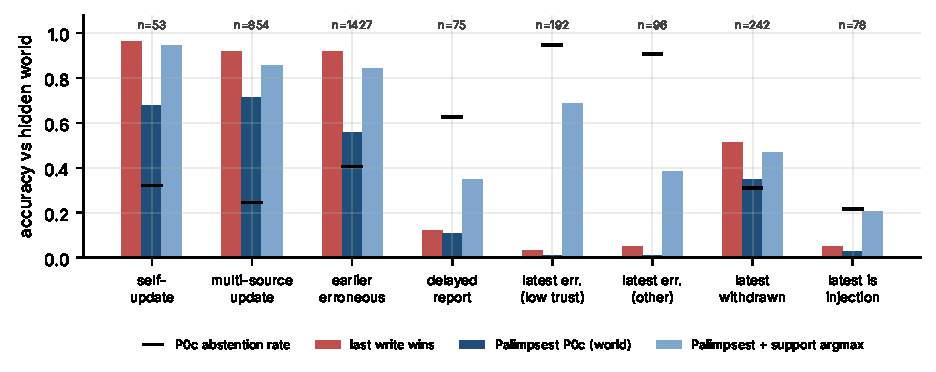
\includegraphics[width=\textwidth]{figures/regime.pdf}
\caption{Accuracy against the hidden world by regime (what the latest report on the key is), value queries on single-valued keys of the 200 fresh streams; poisoning from 60 attack streams. Bars: last-write-wins, \pal{} under P0c, and \pal{} with support-ranked commitment on unresolved slots; ticks: P0c abstention rate.}\label{fig:regime}
\end{figure}
Justified belief is scored against the evidence, but the world is what a user cares about, and the generator knows it. Table~\ref{tab:regime} classifies every value query on a single-valued key of 200 fresh streams by what the latest report on that key is, using the hidden labels, and scores each system against the hidden world value, with P0c and the self-update variant P0cSU on the same queries (the 500 frozen Setting 1 streams give the same picture, Appendix~\ref{app:tables}, Table~\ref{tab:regime-s1}). The pattern is simple. Where the latest report is true---the same origin updating itself (self-update, \rgSelfN{} queries), several origins reporting a change (\rgMultiN), or an earlier report being the erroneous one (\rgStaleN)---last-write-wins is right on \rgSelfLww, \rgMultiLww{} and \rgStaleLww{} of queries and P0c abstains on \rgSelfAbst, \rgMultiAbst{} and \rgStaleAbst{} of them, committing to a non-world value on at most \rgMultiWrong. Where the latest report is wrong---it reports an older fact late (\rgDelayN), or is erroneous from a low-trust (\rgLowN) or another (\rgOthN) source---recency is right on \rgDelayLww, \rgLowLww{} and \rgOthLww, P0c abstains on \rgDelayAbst, \rgLowAbst{} and \rgOthAbst{} and commits to a non-world value on \rgDelayWrong, \rgLowWrong{} and \rgOthWrong. After a withdrawal of the latest report (\rgRetrN) both are near chance against the world because the generator withdraws true reports too: the justified value and the world value come apart by construction. The three ``latest true'' regimes hold \rgLatestTruePct\% of the queries in our generator and the three ``latest wrong'' regimes \rgLatestWrongPct\%; the semantics' refusal to assume recency is paid in the former and earns its keep in the latter.

The poisoning regime is reported as attack-success events, not accuracy. On the \rgPoisN{} queries of the attack streams whose latest report is an injection, last-write-wins by construction commits to the injected value on every query (\rgPoisLwwInj); P0c commits to it on \rgPoisPalInj{} of them and abstains on \rgPoisPalAbst{} (its world accuracy, \rgPoisPalWorld, counts the few injections that happen to be true); support-ranked commitment commits to it on \rgPoisArgmaxInj. Cue resolution (A-CUE) lets a report carrying a false change cue shield itself from its competitors, so the justification layer offers little protection against an attacker who knows the cue vocabulary.

Two consequences were drawn and pre-registered before being tested (Appendix~\ref{app:chronology}), and Table~\ref{tab:regime} reports them paired on the same queries. First, the self-update rule A-SU removes P0c's abstention in the self-update regime (\suFaSelfAbst{} $\to$ \suFbSelfAbst, world accuracy \suFaSelfWorld{} $\to$ \suFbSelfWorld{} $=$ last-write-wins \suFbSelfLww) and raises commitments to non-world values in the delayed and erroneous regimes by 1.3, 1.0 and 0.0 points (\suFaDelayWrong{} $\to$ \suFbDelayWrong, \suFaLowWrong{} $\to$ \suFbLowWrong, \suFaOthWrong{} $\to$ \suFbOthWrong), leaving the propagation effect unchanged ($+\suFaProp$ vs $+\suFbProp$ points); the three pre-stated tests P-A1--P-A3 held (the pre-stated cost bound was 5 points; the paired per-regime differences are in Table~\ref{tab:regime}), the fourth item P-A4 was a mechanism check on already-seen LongMemEval items and not a test, and the rule is adopted with that trade-off stated; the exploratory LongMemEval variant of \S\ref{sec:res-lme} preceded the rule and is distinct from it. Second, graded commitment: committing on an unresolved slot to the alternative with the highest support (\S\ref{sec:support}) is right against the world on \rgArgmaxFull{} of the \rgDisputedN{} disputed queries at full coverage against \rgLwwFull{} for recency on the same queries, and on \rgHalfArgmax{} against \rgHalfLww{} at \rgHalfCov{} coverage when ranked by support margin; per regime it beats recency only where the latest report is wrong (\rgDelayArgmax{} vs \rgDelayLww, \rgLowArgmax{} vs \rgLowLww) and loses where it is right (\rgStaleArgmax{} vs \rgStaleLww). Provenance-and-recency support is therefore not a better committer than recency on average; its value is selective, and that is the form in which it should be used.

\subsection{Setting 2: natural language, automatic extraction}\label{sec:res-s2}
\begin{sidewaystable}\centering\footnotesize\setlength{\tabcolsep}{3.5pt}
\caption{Setting 2 (natural-language streams, automatic extraction with Claude Haiku 4.5; 100 streams, 99 with a warranted downstream query). Stream-level means with 95\% cluster-bootstrap intervals; cost is measured tokens (input $+8\times$ output) per stream.}\label{tab:s2}
\begin{tabular}{lccccccc}
\toprule
System & Warr.\ downstream & Warr.\ direct & Resolvable & Unresolved & Commit rate$\downarrow$ & Prov.\ P & Cost (tok/stream) \\
\midrule
\textsc{Palimpsest} & 0.956 {\tiny[0.93,0.98]} & 0.996 {\tiny[0.99,1.00]} & 0.976 {\tiny[0.97,0.98]} & 0.834 {\tiny[0.80,0.87]} & 0.080 {\tiny[0.06,0.10]} & 0.978 {\tiny[0.97,0.98]} & 188k \\
\quad no propagation & 0.749 {\tiny[0.70,0.79]} & 0.996 {\tiny[0.99,1.00]} & 0.920 {\tiny[0.91,0.93]} & 0.813 {\tiny[0.78,0.85]} & 0.079 {\tiny[0.06,0.10]} & 0.972 {\tiny[0.97,0.98]} & 188k \\
\quad forced commit & 0.979 {\tiny[0.96,0.99]} & 0.996 {\tiny[0.99,1.00]} & 0.987 {\tiny[0.98,0.99]} & 0.045 {\tiny[0.03,0.06]} & 0.758 {\tiny[0.73,0.79]} & 0.985 {\tiny[0.98,0.99]} & 188k \\
Symbolic replay (rule adjudicator) & 0.956 {\tiny[0.93,0.98]} & 0.996 {\tiny[0.99,1.00]} & 0.976 {\tiny[0.97,0.98]} & 0.834 {\tiny[0.80,0.87]} & 0.080 {\tiny[0.06,0.10]} & 0.989 {\tiny[0.99,0.99]} & 188k \\
Claims log + LLM adjudicator & 0.514 {\tiny[0.46,0.56]} & 0.731 {\tiny[0.69,0.77]} & 0.666 {\tiny[0.64,0.69]} & 0.128 {\tiny[0.11,0.15]} & 0.572 {\tiny[0.53,0.61]} & 0.747 {\tiny[0.73,0.76]} & 532k \\
\quad top-40 entries (original, 30 str.) & 0.419 {\tiny[0.32,0.52]} & 0.731 {\tiny[0.64,0.81]} & 0.614 {\tiny[0.57,0.66]} & 0.103 {\tiny[0.08,0.13]} & 0.504 {\tiny[0.46,0.54]} & 0.758 {\tiny[0.73,0.78]} & 454k \\
Raw-report log + LLM adjudicator (30 str.) & 0.330 {\tiny[0.24,0.43]} & 0.685 {\tiny[0.59,0.78]} & 0.554 {\tiny[0.51,0.60]} & 0.101 {\tiny[0.07,0.13]} & 0.606 {\tiny[0.55,0.66]} & 0.683 {\tiny[0.66,0.71]} & 439k \\
Claims log + LLM adj.\ (amended contract, 30 str.) & 0.400 {\tiny[0.33,0.47]} & 0.703 {\tiny[0.60,0.80]} & 0.607 {\tiny[0.57,0.65]} & 0.134 {\tiny[0.09,0.18]} & 0.533 {\tiny[0.47,0.59]} & 0.714 {\tiny[0.69,0.74]} & 552k \\
\quad top-10 entries & 0.225 {\tiny[0.16,0.29]} & 0.787 {\tiny[0.71,0.86]} & 0.572 {\tiny[0.53,0.62]} & 0.138 {\tiny[0.10,0.17]} & 0.377 {\tiny[0.33,0.43]} & 0.836 {\tiny[0.82,0.85]} & 399k \\
\quad top-20 entries & 0.385 {\tiny[0.30,0.48]} & 0.723 {\tiny[0.63,0.81]} & 0.610 {\tiny[0.57,0.65]} & 0.136 {\tiny[0.10,0.18]} & 0.412 {\tiny[0.36,0.46]} & 0.786 {\tiny[0.77,0.80]} & 424k \\
\quad top-40 entries & 0.429 {\tiny[0.33,0.53]} & 0.739 {\tiny[0.65,0.82]} & 0.628 {\tiny[0.59,0.67]} & 0.133 {\tiny[0.10,0.17]} & 0.471 {\tiny[0.42,0.52]} & 0.748 {\tiny[0.73,0.77]} & 464k \\
Raw-report log + LLM adj.\ (amended, 30 str.) & 0.323 {\tiny[0.23,0.42]} & 0.672 {\tiny[0.59,0.76]} & 0.524 {\tiny[0.48,0.57]} & 0.102 {\tiny[0.07,0.14]} & 0.563 {\tiny[0.51,0.61]} & 0.674 {\tiny[0.65,0.70]} & 448k \\
Temporal DB & 0.779 {\tiny[0.74,0.82]} & 0.885 {\tiny[0.85,0.92]} & 0.895 {\tiny[0.88,0.91]} & 0.000 {\tiny[0.00,0.00]} & 0.837 {\tiny[0.81,0.87]} & 0.961 {\tiny[0.95,0.97]} & 188k \\
Always abstain & 0.000 {\tiny[0.00,0.00]} & 0.000 {\tiny[0.00,0.00]} & 0.000 {\tiny[0.00,0.00]} & 0.380 {\tiny[0.35,0.41]} & 0.000 {\tiny[0.00,0.00]} & 0.542 {\tiny[0.52,0.56]} & 188k \\
Always commit & 0.422 {\tiny[0.38,0.46]} & 0.982 {\tiny[0.97,0.99]} & 0.791 {\tiny[0.77,0.81]} & 0.000 {\tiny[0.00,0.00]} & 0.795 {\tiny[0.77,0.82]} & 0.947 {\tiny[0.94,0.96]} & 188k \\
\bottomrule
\end{tabular}
\end{sidewaystable}
\paragraph{Evaluation set and extraction.} 100 streams (13{,}094 reports) were rendered, paraphrased by Claude Haiku 4.5 and passed through the cue-recovery check: 1{,}343 lines were flagged by the model-side check, almost all because a dated statement (``since 3 March'') was read as a change, a reading that cannot alter gold and was counted but not acted on; after two regenerations 56 lines had lost a stated change cue and 3 had gained one, and adjudication stripped the lost cues from the frozen labels, changing 274 of 6{,}737 gold entries (4.1\%). The frozen set has \sTwoWarrPerStream{} warranted downstream queries per stream (741 in 99 streams), under the pre-registered floor of 8 (deviation recorded). The shared extractor (Haiku 4.5) produces one claim per report line; against the frozen labels the errors are, with the line count as denominator: value or entity wrong on \sTwoExtSlot\% (the slot-error rate), a stated operator cue dropped on \sTwoExtMissed\%, a cue added on \sTwoExtSpur\%, a stated date wrong or dropped on \sTwoExtValid\%, no parseable claim on \sTwoExtFail\%; the categories overlap and are not a single rate. No independent human audit of the paraphrases or extractions was performed; the same model family generated, checked, extracted and adjudicated, and correlated misreadings are possible (\S\ref{sec:threats}).

\paragraph{Symbolic maintenance vs LLM adjudication over the same claims.} On warranted downstream queries \pal{} over the extracted claims reaches \sTwoPalWarr{} against \sTwoLogWarr{} for the same claims log adjudicated by the LLM at query time, a paired difference of $+\sTwoHOne$ points $[\sTwoHOneLo, \sTwoHOneHi]$ over \sTwoHOneN{} streams. Symbolic replay over the same claims reaches \sTwoRuleWarr{}, identical to \pal, so the gap is between the rule engine and the prompted adjudicator, not between write time and query time. We do not attribute it to ``reasoning'': the measured categories are a scoring convention the adjudicator was not told (\primEmpty{} of the \primN{} primary queries have empty-set gold; its micro accuracy is \primLogExact{} with them and \primLogExactNe{} without), established-false and unresolved-set answers it renders as \emph{unknown}, and inferences it does not make; Appendix~\ref{app:errors} gives the rule-coded taxonomy over the 4{,}062 primary answers: 15.7\% premature commitments, 9.8\% under-commitments with the gold value among the listed alternatives, 8.2\% wrong alternative sets, 6.0\% wrong committed values, 6.5\% answers on slots whose gold is \texttt{unknown}, and 3.0\% convention cases. Removing propagation costs $\sTwoProp$ points $[\sTwoPropLo, \sTwoPropHi]$, the same effect as in Setting 1.

\paragraph{Amended contract and the context-budget curve (one common subset).} The scoring contract as run did not state the empty-set convention (\S\ref{sec:semantics}). We froze a corrected contract after the original runs and reran every LLM baseline on one common subset, the first \sTwoSubN{} streams, keeping the original-protocol results as such (Appendix~\ref{app:chronology}). On that subset \pal{} scores \sTwoSubPalWarr{} and the original-protocol adjudicator \sTwoSubLogWarr{} (paired $+\sTwoSubLogDiff$ $[\sTwoSubLogDiffLo, \sTwoSubLogDiffHi]$); under the amended contract the adjudicator scores \sTwoCtwoLogWarr{} (paired $+\sTwoCtwoLogDiff$ $[\sTwoCtwoLogDiffLo, \sTwoCtwoLogDiffHi]$), with resolvable accuracy \sTwoCtwoLogRes{} and commitment on \sTwoCtwoLogCommit{} of unresolved slots. The context-budget variants, which show the adjudicator the $k$ most recent entries plus every entry on the queried key, score \sTwoCtwoTopTenWarr{} ($k=10$, \sTwoCtwoTopTenTok{}k tokens per stream), \sTwoCtwoTopTwentyWarr{} ($k=20$, \sTwoCtwoTopTwentyTok{}k) and \sTwoCtwoTopFortyWarr{} ($k=40$, \sTwoCtwoTopFortyTok{}k) against \sTwoCtwoLogWarr{} with the full log (\sTwoCtwoLogTok{}k) and \pal's \xE{}k, which is the shared extraction cost alone. The raw-report adjudicator with no extraction scores \sTwoCtwoNlWarr{} at \sTwoCtwoNlTok{}k. A claims-log adjudicator that pays the shared extraction cost cannot be given a budget equal to extraction alone; every budget we could give it costs more than \pal{} and scores lower, so the registered ``matched cost'' test was not executable as written. H1 is supported on accuracy at every budget we ran and is reported as incompletely tested under its registered cost condition; the original-protocol estimate ($+\sTwoHOne$ on 100 streams) and the amended-protocol estimate ($+\sTwoCtwoLogDiff$ on 30) are separate numbers on different populations and are not combined. H2 as registered concerned LLM-token cost: with extraction at \xE{}k weighted tokens per stream and raw-report adjudication at \xAnl{}k per query, write-time extraction becomes cheaper than adjudicating the raw reports at $r^*=\holmHTwoR$ queries per observation [\holmHTwoLo, \holmHTwoHi] (stream-level bootstrap over the 30 raw-report streams), so H2 holds as a token-cost statement; it is a different quantity from the CPU crossover against symbolic replay in \S\ref{sec:res-systems}, and the two should not be read as one result.

\paragraph{Uncertainty and harm.} The LLM adjudicator commits on \sTwoLogCommit{} of unresolved slots against \sTwoPalCommit{} for \pal, while \pal's resolvable accuracy is \sTwoPalRes{} against \sTwoLogRes: both halves of the joint criterion H4 hold (Appendix~\ref{app:tables}, Table~\ref{tab:holm}). The registered ``unsupported propagation'' endpoint is renamed \emph{answer instability under unchanged gold} and decomposed in Table~\ref{tab:trans} on the \trN{} non-warranted event pairs (micro rates over pairs; Table~\ref{tab:s2} gives the stream-level macro average of the same quantity). \pal{} changes its answer on \trPalInst{} of pairs and goes from a correct to a wrong answer on \trPalCW; the adjudicator changes on \trLogInst, goes correct$\to$wrong on \trLogCW, wrong$\to$correct on \trLogWC{} and wrong$\to$wrong on \trLogWW. \pal's correct$\to$wrong transitions are extraction-induced: in 35 of its 37 such pairs a report arriving at the event's belief time was mis-extracted relative to the frozen text, and symbolic replay shows the same rate. An earlier draft reported 0.007 against 0.076 for these two numbers; those were computed against the pre-adjudication gold and are withdrawn. The harm claim is therefore modest: on this measure the adjudicator is less stable by a factor of four and slightly more harmful. The forced-commit variant scores \sTwoCommitWarr{} on warranted queries, above \pal, because committing to the minimal-error interpretation often resolves a spurious dispute created by an extraction error in the right direction, at the price of committing on \sTwoCommitCommit{} of genuinely unresolved slots.
\begin{table}[t]\centering\small
\caption{Answer transitions on the non-warranted event pairs of Setting 2 (frozen gold unchanged between $\tau-1$ and $\tau$; micro rates over pairs). C = exact match with gold, W = not. Instability is the registered ``unsupported propagation'' metric (answer changed while gold did not); harm is C$\to$W.}\label{tab:trans}
\begin{tabular}{lrcccc c}
\toprule
System & $n$ & C$\to$C & C$\to$W & W$\to$C & W$\to$W & instability \\
\midrule
\textsc{Palimpsest} & 587 & 0.850 & 0.063 & 0.012 & 0.075 & 0.092 \\
\quad no propagation & 587 & 0.819 & 0.061 & 0.034 & 0.085 & 0.107 \\
\quad forced commit & 587 & 0.424 & 0.003 & 0.003 & 0.569 & 0.107 \\
Symbolic replay (rule adjudicator) & 587 & 0.850 & 0.063 & 0.012 & 0.075 & 0.092 \\
Claims log + LLM adjudicator & 587 & 0.206 & 0.080 & 0.032 & 0.681 & 0.404 \\
\quad top-40 entries (original, 30 str.) & 172 & 0.221 & 0.134 & 0.041 & 0.605 & 0.529 \\
Raw-report log + LLM adjudicator (30 str.) & 172 & 0.186 & 0.064 & 0.041 & 0.709 & 0.453 \\
Claims log + LLM adj.\ (amended contract, 30 str.) & 172 & 0.203 & 0.110 & 0.029 & 0.657 & 0.448 \\
\quad top-10 entries & 172 & 0.331 & 0.076 & 0.047 & 0.547 & 0.314 \\
\quad top-20 entries & 172 & 0.250 & 0.099 & 0.070 & 0.581 & 0.483 \\
\quad top-40 entries & 172 & 0.227 & 0.110 & 0.041 & 0.622 & 0.483 \\
Raw-report log + LLM adj.\ (amended, 30 str.) & 172 & 0.180 & 0.052 & 0.070 & 0.698 & 0.471 \\
Temporal DB & 587 & 0.417 & 0.003 & 0.003 & 0.576 & 0.150 \\
Always abstain & 587 & 0.124 & 0.017 & 0.000 & 0.859 & 0.121 \\
Always commit & 587 & 0.252 & 0.012 & 0.009 & 0.727 & 0.211 \\
\bottomrule
\end{tabular}
\end{table}

\paragraph{Sign stability with a stronger model.} Re-extracting and adjudicating 15 streams with Claude Sonnet 4.6 on the same frozen set (Appendix~\ref{app:tables}) lowers the slot-error rate to \sStrongExtSlot\% and lifts the adjudicator to \sStrongLogWarr{}; \pal{} reaches \sStrongPalWarr{} and the paired difference stays positive, $+\sStrongHOne$ $[\sStrongHOneLo, \sStrongHOneHi]$. This check changes extractor and adjudicator together and does not isolate either.

\paragraph{Extraction noise.}
\begin{figure}[t]\centering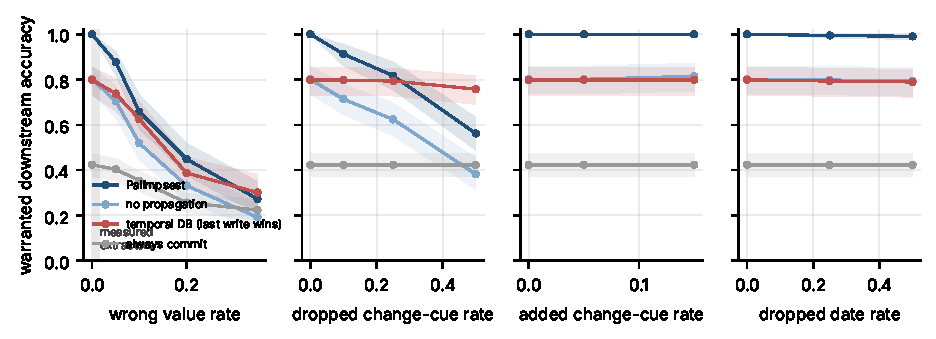
\includegraphics[width=\textwidth]{figures/noise.pdf}
\caption{Warranted downstream accuracy under injected extraction errors (mock extractor, 50 Setting 2 streams; bands are stream-level 95\% bootstrap intervals; the grey band marks the slot-error range of the real extractors, 0.3--1.5\%).}\label{fig:noise}
\end{figure}
Figure~\ref{fig:noise} injects extraction errors at controlled rates. \pal{} degrades faster than last-write-wins as wrong values accumulate: at 20\% wrong values it scores \nzSlotTwentyPal{} against \nzSlotTwentyTdb{} for the temporal DB and at 35\% the order reverses (\nzSlotThirtyfivePal{} vs \nzSlotThirtyfiveTdb); when half the stated change cues are dropped the temporal DB (\nzCueFiftyTdb) is ahead of \pal{} (\nzCueFiftyPal). Every extraction error becomes a standing dispute that the semantics keeps open, whereas last-write-wins discards it. The injected error types are the extractor's measured categories (wrong value, dropped cue, added cue, dropped date), but the rates at which the curves cross are far above the measured ones and are not deployment thresholds.

\subsection{Setting 3: streams derived from Wikidata revision histories}\label{sec:res-s3}
\begin{sidewaystable}\centering\footnotesize\setlength{\tabcolsep}{3.5pt}
\caption{Setting 3 (transfer: 30 streams assembled from Wikidata statement histories, pseudonymised surface, extraction and adjudication with Claude Haiku 4.5). Descriptive; the warranted-downstream stratum has 24 queries in 13 streams.}\label{tab:s3}
\begin{tabular}{lccccccc}
\toprule
System & Warr.\ downstream & Warr.\ direct & Resolvable & Unresolved & Commit rate$\downarrow$ & Prov.\ P & Cost (tok/stream) \\
\midrule
\textsc{Palimpsest} & 0.923 {\tiny[0.77,1.00]} & 0.976 {\tiny[0.94,1.00]} & 0.978 {\tiny[0.95,1.00]} & 0.909 {\tiny[0.73,1.00]} & 0.000 {\tiny[0.00,0.00]} & 0.892 {\tiny[0.85,0.94]} & 25k \\
\quad no propagation & 0.724 {\tiny[0.49,0.93]} & 0.976 {\tiny[0.94,1.00]} & 0.962 {\tiny[0.93,0.99]} & 0.879 {\tiny[0.70,1.00]} & 0.000 {\tiny[0.00,0.00]} & 0.886 {\tiny[0.84,0.93]} & 25k \\
\quad forced commit & 0.923 {\tiny[0.77,1.00]} & 0.976 {\tiny[0.94,1.00]} & 0.978 {\tiny[0.95,1.00]} & 0.000 {\tiny[0.00,0.00]} & 1.000 {\tiny[1.00,1.00]} & 0.892 {\tiny[0.85,0.94]} & 25k \\
Symbolic replay (rule adjudicator) & 0.923 {\tiny[0.77,1.00]} & 0.976 {\tiny[0.94,1.00]} & 0.978 {\tiny[0.95,1.00]} & 0.909 {\tiny[0.73,1.00]} & 0.000 {\tiny[0.00,0.00]} & 1.000 {\tiny[1.00,1.00]} & 25k \\
Claims log + LLM adjudicator & 0.019 {\tiny[0.00,0.06]} & 0.519 {\tiny[0.38,0.66]} & 0.185 {\tiny[0.14,0.23]} & 0.333 {\tiny[0.09,0.61]} & 0.545 {\tiny[0.27,0.79]} & 0.802 {\tiny[0.75,0.86]} & 88k \\
Raw-report log + LLM adjudicator (30 str.) & 0.077 {\tiny[0.00,0.23]} & 0.451 {\tiny[0.30,0.61]} & 0.181 {\tiny[0.13,0.23]} & 0.182 {\tiny[0.00,0.45]} & 0.576 {\tiny[0.30,0.82]} & 0.731 {\tiny[0.67,0.79]} & 71k \\
Claims log + LLM adj.\ (amended contract, 30 str.) & 0.019 {\tiny[0.00,0.06]} & 0.491 {\tiny[0.34,0.64]} & 0.205 {\tiny[0.15,0.26]} & 0.394 {\tiny[0.15,0.64]} & 0.485 {\tiny[0.21,0.73]} & 0.791 {\tiny[0.73,0.85]} & 92k \\
Raw-report log + LLM adj.\ (amended, 30 str.) & 0.173 {\tiny[0.00,0.38]} & 0.466 {\tiny[0.32,0.61]} & 0.208 {\tiny[0.15,0.26]} & 0.318 {\tiny[0.09,0.59]} & 0.439 {\tiny[0.18,0.70]} & 0.728 {\tiny[0.67,0.79]} & 25k \\
Temporal DB & 0.865 {\tiny[0.65,1.00]} & 0.884 {\tiny[0.78,0.97]} & 0.692 {\tiny[0.64,0.74]} & 0.000 {\tiny[0.00,0.00]} & 1.000 {\tiny[1.00,1.00]} & 0.922 {\tiny[0.88,0.96]} & 25k \\
Always abstain & 0.000 {\tiny[0.00,0.00]} & 0.000 {\tiny[0.00,0.00]} & 0.000 {\tiny[0.00,0.00]} & 0.788 {\tiny[0.55,1.00]} & 0.000 {\tiny[0.00,0.00]} & 0.828 {\tiny[0.78,0.88]} & 25k \\
Always commit & 0.000 {\tiny[0.00,0.00]} & 0.506 {\tiny[0.36,0.65]} & 0.478 {\tiny[0.43,0.53]} & 0.000 {\tiny[0.00,0.00]} & 0.909 {\tiny[0.73,1.00]} & 0.803 {\tiny[0.75,0.86]} & 25k \\
\bottomrule
\end{tabular}
\end{sidewaystable}
Setting 3 uses the only data in the study whose conflicts and withdrawals we did not generate: streams \emph{derived from independently authored Wikidata revision histories under an author-defined mapping}. Forty persons selected by a query for histories with deprecated statements and ended employments, and the 128 organisations recorded as their employers, were fetched (3{,}474 sampled revisions; intermediate edits between sampled revisions collapse into one diff) and mapped as follows: a claim added is an assertion (with a \emph{since} cue when it carries a start qualifier), a value edited in place is a correction, a statement deprecated or removed by the editors is a withdrawal; references give the source class (331 of 417 assertions are unreferenced, class \emph{low}); the surface is pseudonymised with the fictional names of Settings 1--2 and the dates are real. The target is editorial state, not the world: a deprecation is scored as a withdrawal of evidence, not as proof that a relationship ended. Three mappings were tried and are reported together: with \emph{employer} single-valued, 1 warranted downstream query in 30 streams; multi-valued and changeable, 4; multi-valued and stable (an affiliation set, which is what the property records), \sThreeWarrTotal{} in 13 streams. The third was adopted and frozen before the LLM runs; it is a consequential, author-made choice, and the setting is exploratory transfer. Two of the 128 organisations appear in more than one stream, so the streams are nearly disjoint and the stream-level bootstrap is appropriate.

\pal{} over the extracted claims reaches \sThreePalWarr{} on the \sThreeWarrTotal{} warranted downstream queries, equal to symbolic replay (\sThreeRuleWarr): the ceiling set by extraction (slot-error rate \sThreeExtSlot\%). Removing propagation costs $\sThreeProp$ points $[\sThreePropLo, \sThreePropHi]$ over 13 streams, a suggestive rather than broad confirmation. The LLM adjudicator reaches \sThreeLogWarr{} on the same queries and \sThreeLogRes{} on resolvable ones under the original contract, and \sThreeCtwoLogWarr{} and \sThreeCtwoLogRes{} under the amended one, so the missing convention explains little of this gap; what does is that \sThreeEstEmpty{} of the \sThreeEstTotal{} established primary queries are empty sets and \sThreeHoldsFalse{} are established-false, on which it answers \emph{unknown}, and that on the warranted queries it answers \emph{unresolved} with the gold set among its alternatives, reasoning that overlapping affiliations ``may have ended'' against a schema that declares the attribute stable. The pseudonymised schema puts the adjudicator's priors against a declaration it was told to follow; that is a limitation of this transfer design as much as of the adjudicator, and the propagation ablation and the equality with replay are the parts of Setting 3 we would rely on.

\subsection{External check: LongMemEval knowledge updates}\label{sec:res-lme}
\begin{table}[t]\centering\footnotesize
\caption{LongMemEval knowledge-update items (78; 69 mapped to an extracted attribute). Systems answer one structured slot from claims extracted turn by turn; a Haiku judge compares the answer with the reference. Coverage = share answered as established; accuracy over all items and over answered items. Not comparable to published LongMemEval scores.}\label{tab:lme}
\begin{tabular}{lccc}
\toprule
System & Coverage & Acc.\ (all) & Acc.\ (answered) \\
\midrule
\pal{} (P0c) & 0.32 & 0.167 & 0.400 \\
\pal{} + self-update (exploratory) & 0.74 & 0.474 & 0.621 \\
Temporal DB (last write wins) & 0.88 & 0.526 & 0.594 \\
Always-commit & 0.88 & 0.526 & 0.594 \\
Always-abstain & 0.00 & 0.038 & 0.000 \\
Claims log + LLM adjudicator & 0.56 & 0.359 & 0.614 \\
\bottomrule
\end{tabular}
\end{table}
LongMemEval's knowledge-update items \citep{longmemeval} ask for a user attribute stated and later updated across chat sessions. We run the \lmeN{} items of the oracle release (cleaned version of 3 October 2026; sessions are not chronologically ordered in the release and are sorted by their timestamps before belief time is assigned) through an open-vocabulary adapter shared by all systems: each user turn is extracted into claims about the user, attribute keys are canonicalised per item, the question is mapped to one key, every system answers that slot, and a model judge compares the answer with the reference; abstention is credited on the six items whose reference is ``not enough information''. The adapter caps every system (9 items map to no key; always-abstain scores 3/78 because three abstention items are among the unmapped) and the numbers are not comparable to published LongMemEval scores.

Two things are measured at once and we separate them. The benchmark's reference for an update is the user's \emph{latest} statement: it tests the self-update regime of Table~\ref{tab:regime} and only that regime. Under P0c a later uncued value from the same source is a dispute, so \pal{} answers \emph{unresolved} on \lmePalUnres{} of 69 mapped items (coverage \lmePalCov, accuracy \lmePalAcc), where last-write-wins answers and is right on 34 of them (\lmeTdbAcc{} at coverage \lmeTdbCov); on items where both commit they agree, and support-ranked commitment reproduces last-write-wins exactly, because with a single source support reduces to recency. The adapter is the other limit: the extractor recovered a stated change on 5 of 91 claims on the queried keys, questions about previous values or about the change itself cannot be expressed in a single current-value slot, and the LLM adjudicator abstains on 44\% (\lmeLogAcc). The pre-registered self-update rule, applied to these already-seen items as a mechanism check only, gives \lmePalSuAcc{} at coverage \lmePalSuCov. Our reading: a policy that requires explicit change cues loses coverage wherever updates arrive as ordinary self-reports, which is a practical limitation of P0c and the reason A-SU is now the default for self-report streams; and what this benchmark does not contain---unreliable sources, hidden world state, withdrawn evidence---is what the other settings measure. STALE \citep{stale2026} was not evaluated: at the time of our runs we could not reach a data release, and its native question interface at 100K-token contexts exceeded the remaining budget; a public repository has since been reported and the evaluation is left for a later version.

\subsection{Calibrated support and poisoning}\label{sec:res-rq3}
\begin{table}[t]\centering\small
\caption{RQ3, Setting 1 (held-out streams): claim-level calibration of support against the hidden world. Lower is better.}\label{tab:rq3}
\begin{tabular}{lccc}
\toprule
Confidence & Brier & ECE & AURC \\
\midrule
Evidence model, declared priors & 0.182 & 0.118 & 0.138 \\
Evidence model, learned class priors & 0.175 & 0.113 & 0.131 \\
\quad without origin grouping & 0.179 & 0.121 & 0.136 \\
\quad without recency & 0.236 & 0.202 & 0.156 \\
\quad without cue adjustments & 0.183 & 0.128 & 0.136 \\
Class prior only & 0.255 & 0.227 & 0.168 \\
Logistic regression on evidence features & 0.138 & 0.034 & 0.112 \\
Constant 0.5 & 0.250 & 0.496 & 0.268 \\
\bottomrule
\end{tabular}
\end{table}
Support (\S\ref{sec:support}) is a weighted log-odds rule, auditable but not a fitted model, and it predicts a defined event: that a candidate value is the world value at the query's valid time. On 200 held-out Setting 1 streams (\RqN{} candidate values) with class priors learned on 300 training streams it has ECE \RqLearnedEce{} and Brier \RqLearnedBrier, against \RqPriorEce{} and \RqPriorBrier{} for class priors alone, and against \RqLogregEce{} and \RqLogregBrier{} for a logistic regression over the same evidence features trained on the same streams; recency is the largest single contributor (ECE \RqNoRecEce{} without it). In Setting 2, on the \RqTwoSupN{} value queries the LLM adjudicator answered as established and the same asserted values, support has ECE \RqTwoSupEce{} against \RqTwoVerbEce{} for the adjudicator's verbalised confidence and \RqTwoSampEce{} for agreement across five samples on a 300-query subset (risk--coverage areas \RqTwoSupAurc, \RqTwoVerbAurc, \RqTwoSampAurc). H3 is not supported: a provenance-and-recency rule is less well calibrated than a learned predictor and than the adjudicator's own confidence on these populations. The selection by the adjudicator's established answers and the smaller sampling subset are reported as such; reliability diagrams are in Appendix~\ref{app:tables} (Figure~\ref{fig:rel}).
\begin{table}[t]\centering\small
\caption{Poisoning (Setting 1, 60 streams per cell). Attacker injects false assertions at a rate of the honest ones, half with a false change cue; harm = share of value queries answered \emph{established} with the poisoned value; support = mean support the evidence model assigns to poisoned vs.\ honest candidates.}\label{tab:poison}
\begin{tabular}{llcccccc}
\toprule
Channel & Rate & \multicolumn{2}{c}{\textsc{Palimpsest}} & \multicolumn{2}{c}{Temporal DB} & \multicolumn{2}{c}{Support} \\
 & & harm$\downarrow$ & unresolved & harm$\downarrow$ & unresolved & poisoned & honest \\
\midrule
low & 0.01 & 0.003 & 0.27 & 0.003 & 0.03 & 0.21 & 0.67 \\
low & 0.05 & 0.024 & 0.28 & 0.030 & 0.03 & 0.33 & 0.67 \\
low & 0.20 & 0.112 & 0.30 & 0.151 & 0.03 & 0.32 & 0.65 \\
trusted & 0.01 & 0.005 & 0.27 & 0.005 & 0.03 & 0.63 & 0.67 \\
trusted & 0.05 & 0.027 & 0.28 & 0.033 & 0.03 & 0.66 & 0.66 \\
trusted & 0.20 & 0.115 & 0.30 & 0.153 & 0.03 & 0.63 & 0.63 \\
\bottomrule
\end{tabular}
\end{table}
Under the explicit attacker model (Table~\ref{tab:poison}), at 20\% injection through a low-trust channel \pal{} answers established with the poisoned value on \PoisHarmPal\% of value queries against \PoisHarmTdb\% for the temporal DB, and the support layer separates poisoned from honest candidates through the low channel (mean support \PoisSupLowPois{} vs \PoisSupLowHon) but not through a compromised trusted one (\PoisSupTrPois{} vs \PoisSupTrHon): provenance cannot detect what provenance has endorsed. The regime view (\S\ref{sec:res-regime}) adds the conditional number: when the latest report is the injection, \pal{} commits to the injected value on \rgPoisPalInj{} of queries.
